\documentclass[logo,reportComp]{thesis}
\usepackage[cpp,pseudo]{mypackage}

\title{操作系统原理实验报告}
\subtitle{实验五:系统中断}
\school{数据科学与计算机学院}
\author{陈鸿峥}
\classname{17大数据与人工智能}
\stunum{17341015}
\headercontext{操作系统原理实验报告}
% \authorremark{本实验报告用\LaTeX撰写,创建时间:\builddate\today}

\begin{document}

\maketitle

\section{实验目的}
\begin{itemize}
	\item 明白系统调用的意义并设计一组系统调用功能
\end{itemize}

\section{实验要求}
% 实验目的和实验要求由老师提供实验项目文档中获取
\begin{itemize}
	\item 增加一组系统调用,采用功能号实现
	\item 设计C程序库以调用这组系统调用
\end{itemize}

\section{实验环境}
% 包括:硬件或虚拟机配置方法、软件工具与作用、方案的思想、相关原理、程序流程、算法和数据结构、程序关键模块,结合代码与程序中的位置位置进行解释。不得抄袭,否则按作弊处理。
% 实验方案包括相关基础原理、实验工具和环境、程序流程和算法思想、数据结构与程序模块功能说明,代码文档组成说明等
具体环境选择原因已在实验一报告中说明。
\begin{itemize}
	\item Windows 10系统 + Ubuntu 18.04(LTS)子系统
	\item gcc 7.3.0 + nasm 2.13.02 + GNU ld (Binutils) 2.3.0
    \item GNU Make 4.1
	\item Oracle VM VirtualBox 5.2.8
    \item Bochs 2.6.9
	\item Sublime Text 3
\end{itemize}

虚拟机配置:内存4M,无硬盘,1.44M虚拟软盘引导。

\section{实验方案}
% 包括:主要工具安装使用过程及截图结果、程序过程中的操作步骤、测试数据、输入及输出说明、遇到的问题及解决情况、关键功能或操作的截图结果。不得抄袭,否则按作弊处理。
\subsection{系统调用}
因为操作系统要提供的服务非常多,服务子程序数量太多,但中断向量有限,因此,实际做法是专门指定一个中断号对应服务处理程序总入口,然后再将所有服务用功能号区分,并作为一个参数从用户中传递过来,服务程序再进行分支,进入相应的功能实现子程序。
规定系统调用服务的中断号是21h。

具体实施中,写了\verb'int 21h'中断,通过\verb'ax'传递功能号(类似读磁盘的中断方法\verb'int 10h')。
目前提供的中断向量功能如下
\begin{center}
\begin{tabular}{|c|c|c|}\hline
中断向量号 & 功能号 & 功能 \\\hline
\multirow{5}{*}{int 21h} & 0 & 返回shell\\\cline{2-3}
& 1 & 调用用户子程序1 \\\cline{2-3}
& 2 & 调用用户子程序2 \\\cline{2-3}
& 3 & 调用用户子程序3 \\\cline{2-3}
& 4 & 调用用户子程序4 \\\hline
\end{tabular}
\end{center}

整合后的测试系统调用例子如下(用户子程序5)
\begin{lstlisting}[language={[x86masm]Assembler}]
start:
	mov ax, 1
	int 21h
	mov ax, 2
	int 21h
	mov ax, 3
	int 21h
	mov ax, 4
	int 21h
	ret
\end{lstlisting}

\subsection{C输入输出标准库函数}
本次实验实现了C的标准输入输出函数,即\verb'printf'、\verb'scanf'和\verb'sscanf'。
这几个函数其实只是我提供的输入输出系统调用的封装,在C里面对字符串进行处理,在汇编中进行系统调用,基本实现原有C库函数的功能,具体实施见\verb'sysio.h'头文件。
注意这几个函数都是可以\textbf{传递可变参数的},举例来说
\begin{lstlisting}
printf("%s %d %c",str,i,c);
printf("This is a test: %s",str);
\end{lstlisting}
这两者在我的程序中都合法。

同时也增加了大量其他库函数,如
\begin{itemize}
	\item 判断字符/字符串类型:\verb'isdigit'、\verb'isspace'、\verb'isnum'等
	\item 字符串拷贝:\verb'strncpy'、\verb'strmcpy'等
	\item 字符串分割:\verb'split'
	\item 其他字符串函数已在实验三中实现
\end{itemize}

其他库函数请见\verb'\include'文件夹内的头文件。

\subsection{C/Python解释器}
这是本次实验\textbf{最大的亮点},我编写了一个类C/Python的解释器(interpreter),并提供了\textbf{交互界面}。
在该交互界面中可以进行前面说的\textbf{输入输出系统调用},并可以进行\textbf{简单的四则运算},同时\textbf{声明并存储}变量。
具体实施见\verb'interpreter.h',结果见下一节。

测试输入输出函数

\section{实验结果}
执行用户程序5的结果见图\ref{fig:system},即连续调用系统调用,注意用户程序都是\textbf{可再入的}---调用完系统中断后依然能回到断点继续执行。
\begin{figure}[H]
\centering
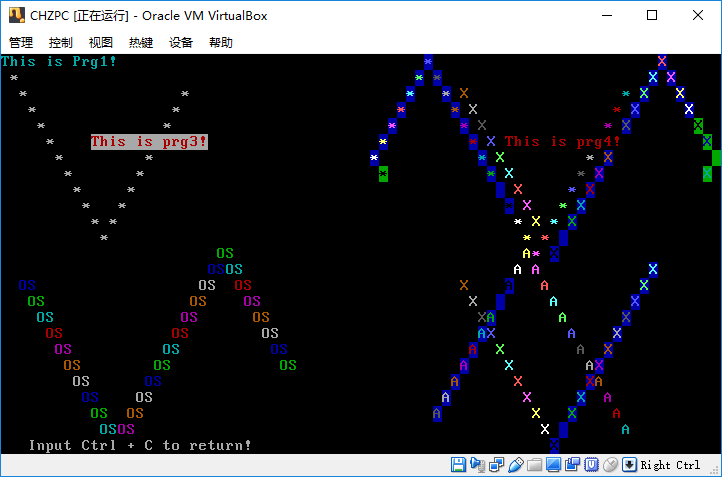
\includegraphics[width=0.8\linewidth]{fig/system.PNG}
\caption{系统调用}
\label{fig:system}
\end{figure}

\verb'scanf'和\verb'printf'的测试函数见下面程序,该函数在\verb'interpreter.h'头文件中。
\begin{lstlisting}
void io_test()
{
	char* str = "This is a scanf test:\n";
	char* format = "%s";
	printf(format, str);
	str = "Please enter two numbers (a and b): ";
	printf(format, str);
	int a, b;
	format = "%d %d";
	scanf(format,&a,&b);
	str = "This is a printf test: ";
	int c = a + b;
	char d = '!';
	format = "%s\nThe sum of a and b is: %d + %d = %d%c\n";
	printf(format, str, a, b, c, d);
}
\end{lstlisting}

实验结果如图\ref{fig:io}所示,注意所有的\verb'scanf'样例都是现场输入的,而不是预先写死在程序中的。
\begin{figure}[H]
\centering
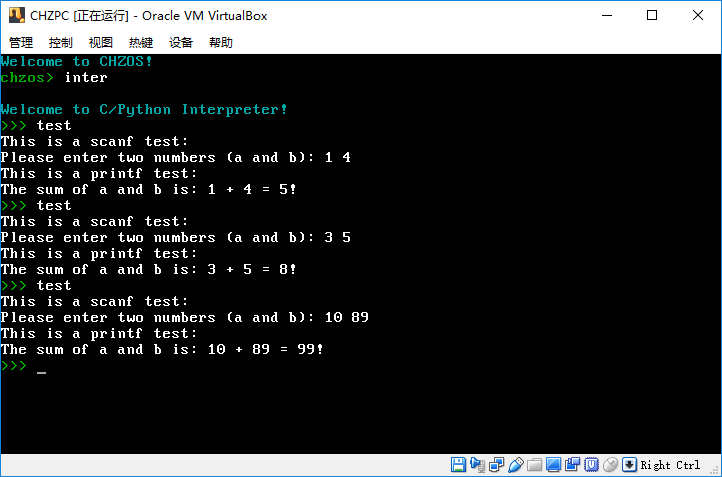
\includegraphics[width=0.8\linewidth]{fig/io.PNG}
\caption{C输入输出函数测试}
\label{fig:io}
\end{figure}

进入解释器的指令为\verb'inter',解释器的实验结果如图\ref{fig:interpreter}所示。
注意
\begin{itemize}
	\item 在数字输入时会直接进行计算
	\item 目前支持简单的四则运算指令
	\item 字母输入默认为指令,若无该条指令则报错
	\item 可以\textbf{声明变量存储}并运算
	\item 基本设置与Python命令行一致
\end{itemize}
\begin{figure}[H]
\centering
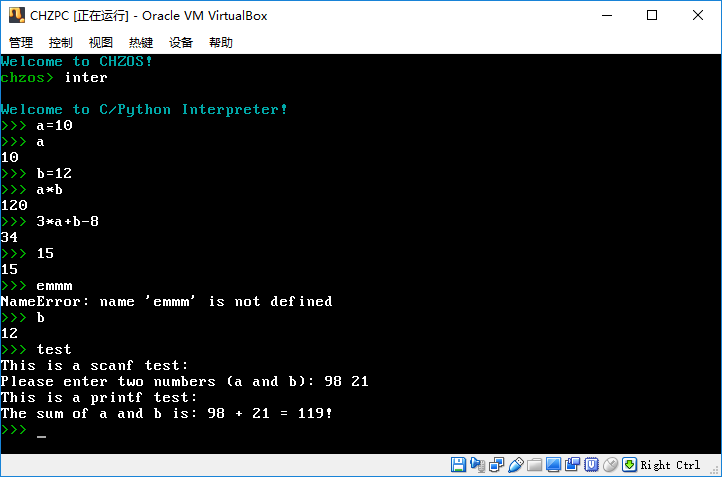
\includegraphics[width=0.8\linewidth]{fig/interpreter.PNG}
\caption{C/Python解释器}
\label{fig:interpreter}
\end{figure}

\section{实验总结}
% 每人必需写一段,文字不少于500字,可以写心得体会、问题讨论与思考、新的设想、感言总结或提出建议等等。不得抄袭,否则按作弊处理。
本次实验并不难,只需将原来的中断调用全部整合入一个系统调用即可,并通过寄存器传递功能号,实现不同的功能。

以前写高级语言程序调试往往通过在自己期望的断点处进行debug输出,但现在当要自己实现输入输出函数时,便没有一个参照物告诉你哪里错了,所以调试难度非常大。
因此,我采用的是核心分离的方法,即用普通的C程序先在正常的电脑上调试输出通过后,再将所有的\verb'printf'函数换回我提供的库函数\verb'putchar'。
这样现在自己电脑上将字符串输入输出函数调试成功后,再放入操作系统,就不会遇到太多问题。
不过要注意由于我现在的内核已经太大了,占了23个扇区,因此加载的用户程序已经不能放在\verb'0A100h',需要另找位置,否则原来的内核会被覆盖,导致无法再入。

为了给自己提升难度,于是我自行设计了一个C的解释器,实际上是类似Python的功能与界面。
由于C是静态语言,所以传统的C程序一定要通过编译,将高级语言程序转换为机器码才可以在机器上运行。
而Python这种动态语言则采用解释器的模式,逐行读取逐行运行。
近年来科学计算比较火的Julia这门语言,现在已经出到1.0版,可以对C程序进行解释执行。
我想既然我要实现操作系统,也要实现命令行界面,那不如也亲自实施一下,看看难度有多大。
实际效果就如实验中所呈现的一样,目前还只能做一些简单的四则运算,之后会添加更多功能。

操作系统这门课真是越来越有趣了,从上层到底层全部打通了,甚至开始自己写编译器/解释器,真不愧是一门系统的课程。

\section{参考资料}
\begin{enumerate}
	\item 李忠,王晓波,余洁,《x86汇编语言-从实模式到保护模式》,电子工业出版社,2013
\end{enumerate}

\appendix
\appendixconfig
\section{程序清单}
\label{sec:code}
由于程序太多,请直接见压缩文件。

\section{附件文件说明}
\begin{center}
\begin{tabular}{|c|l|l|}\hline
序号 & 文件 & 描述 \\\hline
1 & \verb'bootloader.asm' & 主引导程序\\\hline
2 & \verb'os.asm' & 内核汇编部分\\\hline
3 & \verb'kernel.c' & 内核C部分\\\hline
4 & \verb'Makefile' & 编译指令文件\\\hline
5 & \verb'link.ld' & 链接文件\\\hline
6 & \verb'bochsrc.bxrc' & bochs调试文件\\\hline
7 & \verb'mydisk.img' & 核心虚拟软盘\\\hline
8$\thicksim$13 & \verb'prgX.asm' & 用户程序\\\hline
14$\thicksim$19 & \verb'/include' & 内核头文件\\\hline
\end{tabular}
\end{center}

\end{document}

% 实验提交内容
% 实验报告:电子版(Word2003的DOC格式或PDF格式)
% 原程序文件及可执行代码程序文件
% 测试输入数据文件和输出数据文件
% 虚拟机软盘映像文件

% 基础实验项目5个和扩展实验7个
% 实验项目,迟交影响成绩评价!
% 工具与环境可由选择,开发新型工具或优化一套开发环境都可加分!
% 一系列基础实验项目必须连续完成,当前项目只能在前一个项目的基础上进行,体现出前后的进化关系,否则要被约谈,证明没有抄袭行为!
% 一个项目可提交多个改进的版本,实现新功能和个性化特征都有利于提高相应项目的成绩。
% 实验项目提交内容用winrar工具整体压缩打包,统一格式命名为:
%    <学号>+<姓名>+<实验项目号>+<版本号>.rar
%    姓名(学号)实验NvX.zip
%    实验报告、项目文件夹、映像文件
%    ftp://172.18.216.232 sysuac 下周六23:59

% 免考
% 条件:实验1~6全部评价AAAAB+B+或相当
% 最终成绩可能范围:75分以上